\begin{chapterquote}
 ``It is amusing to note that fluid equations were developed originally to
 simplify the discrete equations of individual particle dynamics. Now we must
 reformulate the continuum problem to solve equations for finite volumes of material.''
 \quoteauthor{Elaine Oran and Jay Boris}
\end{chapterquote}

\chapter{Numerical method}
\label{chapter:numerical_method}

\section{Overview}

This chapter outlines the numerical method used to solve the FANS governing equations
shown in the previous chapter. The ``overlines'' and
``tildes'' used to denote time-averaged properties in the previous chapter
are dropped here for convenience. All derivatives appearing in the diffusion,
source, and metrics terms are approximated using centered second-order accurate
finite-difference stencils, while the convection derivative is modeled through
the Yee-Roe \cite{book:1998:laney} scheme. A block implicit approximate factorization
algorithm solves the discretized form of the residual to steady-state with
the use of a CFL-based local pseudotime step. Also, a novel convergence acceleration
algorithm based on domain decomposition is presented, named the marching window.
The marching window is shown to decrease the work needed to
reach steady-state by $\sim 10$ times for several viscous hypersonic problems
involving large streamwise recirculation regions.



\section{Exact form of the residual}

The residual of the full Navier-Stokes equations
can be expressed in generalized coordinates in tensor
form for any number of dimensions as
%
\begin{equation}
 \frameeqn{
 R=
     \sum_{i=1}^{\nd}
      \left[ \frac{\partial {F_i}}{\partial X_i}
            - \sum_{j=1}^{\nd} \frac{\partial }{\partial X_i}
             \left( K_{ij} \frac{\partial G}{\partial X_j}\right) \right]
     -S
 }~,
  \label{eqn:residual}
\end{equation}
%
where the minimization of $R$ is sought and where $d$ refers to the number of dimensions.
Due to the non-linearity of the system of equations,
a fictitious unsteady term ${\partial Q}/{\partial \pseudot}$
is necessary to obtain the right physical root from a given set of initial conditions,
\ie
%
\begin{equation}
 \frac{\partial Q}{\partial \pseudot} =-R \, .
\end{equation}
%
Even though the numerical methods outlined in this chapter
(including the spatial and temporal discretization along with
the pseudotime stepping schemes) are
not linked to some governing equations in particular,
this study focuses on the Favre averaged Navier-Stokes equations (FANS)
closed by the Wilcox $k\omega$ model \cite{aiaa:1988:wilcox} shown in the
previous chapter.
The vectors $Q$, $F$, $G$ and the conductivity matrix $K$ part
of the RHS of Eq.~(\ref{eqn:residual}) can be obtained from ...
and ...
The source term $S$ is composed of the sum of
a modification to the baseline Wilcox $k\omega$ source terms outlined
in Eq.~... with the dilational dissipation $\epsilon_d$
and an unsteady source term,
%
\begin{equation}
  S=
  \frac{1}{J} \left[
  \begin{array}{c}
    \vdots \alb
    0 \alb
    P_k- \rho k \omega  -\rho \epsilon_d \alb
    \bigfrac{\omega}{\widetilde{k}}\left(
      {\mfc\frac{5}{9}} P_k - {\mfc\frac{5}{6}} \rho k \omega
      + \rho \epsilon_d
    \right)
  \end{array}
  \right]
  - \frac{\partial Q}{\partial t} \, ,
\end{equation}
%
where the turbulent kinetic energy production term was defined previously
in Eq.~...
It is noted that in the Wilcox $k\omega$ model, $\widetilde{k}$ is
set simply to $k$ which in the freestream is set to a small
value to prevent a division by zero. We prefer, however, to specify
$k=0$  in the freestream and, in order to prevent a division by zero
in the dissipation rate source term, to define $\widetilde{k}$ as
%
\begin{equation}
  \widetilde{k}={\rm max}\left[ k ~,~~\min \left(k_{\rm div}~,
                 ~~\frac{\omega \mu} {\rho}\right)\right] \, ,
  \label{eqn:ktilde}
\end{equation}
%
with $k_{\rm div}$ a user-specified constant which is generally set lower than
one tenth of the maximum value of $k$ throughout the boundary layer. This is
verified numerically not to affect the laminar sublayer
but to improve the robustness and efficiency of the integration significantly.
The minimum between $k_{\rm div}$ and $\omega \mu / \rho$ is taken so that a
clipping occurs \emph{only} in non-turbulent flow regions in which an accurate
representation of $\omega$ does not affect the accuracy of the flowfield.




\section{Discretized form of the residual}

The discretization of all terms in the residual is now presented.
By referring to the discretized form of the derivatives along the
$X_i$ coordinate by $\delta_{X_i}$, the discretized residual
$R_\Delta$ can be written as
%
\begin{equation}
\frameeqn{
R_\Delta = \sum_{i=1}^{\nd}  \left[
   \delta_{X_i} F_i -
       \sum_{j=1}^{\nd}
      \delta_{X_i} \left( K_{ij} \delta_{X_j} G\right)
   \right] -S_\Delta
}~,
\label{eqn:resdelta}
\end{equation}
%



\subsection{Diffusion terms}

The
use of tensor form in writing the governing equations in curvilinear
coordinates shown in Eq.~(\ref{eqn:residual}), along with the unique compact
$K_{ij}$ matrix described in Eq.~(...), simplify greatly the discretization
and practical implementation of the viscous terms: less than 100 lines of code are
needed to implement the viscous contribution of the residual for all $d \in [1,~2,~3]$.
Using second-order accurate
centered finite difference stencils, the discretization of the viscous terms,
with $i=j$, corresponds to
%
\begin{equation}
 \frameeqn{
\left[ \delta_{X_i} \left( {K_{ii}}\delta_{X_i} G \right) \right]^{X_i}
 =K_{ii}^{X_i+\frac{1}{2}} \left( G^{X_i+1}-G^{X_i} \right)-
  K_{ii}^{X_i-\frac{1}{2}} \left( G^{X_i}-G^{X_i-1} \right)
 }~,
\end{equation}
%
and, with $i \neq j$, corresponds to,
%
\begin{equation}
 \frameeqn{
 \begin{array}{l}
   \left[ \delta_{X_i}\left( K_{ij}\delta_{X_j} G \right) \right]^{X_i,X_j}\alb
   \begin{array}{rl}
 ~=\!\!&\!\!\! \frac{1}{4} K_{ij}^{X_i+\frac{1}{2},X_j} \left(G^{X_i,X_j+1}+G^{X_i+1,X_j+1} -G^{X_i,X_j-1}-G^{X_i+1,X_j-1}  \right) \alb
 ~-\!\!&\!\!\! \frac{1}{4} K_{ij}^{X_i-\frac{1}{2},X_j} \left(G^{X_i-1,X_j+1}+G^{X_i,X_j+1} -G^{X_i-1,X_j-1}-G^{X_i,X_j-1}  \right)
   \end{array}
 \end{array}
 }~,
\end{equation}
%
where $K^{X_i+\frac{1}{2}}$ midway between nodes is
taken as half the value of $K^{X_i+1}$ and $K^{X_i}$ for example.



\subsection{Convection terms: Yee-Roe flux limited method}

The Yee-Roe flux-limited method here refers to the second-order extension
of the Roe scheme \cite{jcp:1981:roe} by
the Yee limiters applied to the characteristic variables \cite{jcp:1990:yee}.
The first-order accurate Roe scheme is itself a generalization to
a system of multiple equations of
the Courant upwinded scheme \cite{misc:1952:courant} for a scalar advection equation,
which can be written as
%
\begin{equation}
  a\frac{\partial q}{\partial X_i} \approx
  a \left\{
    \begin{array}{ll} q^{X_i+1}-q^{X_i} & ~~{\rm if}~a<0 \\
                      q^{X_i}-q^{X_i-1} & ~~{\rm otherwise,}\end{array}
\right.
\end{equation}
%
where the RHS corresponds exactly to
%
\begin{equation}
  \frac{1}{2} \left[
                         a q^{X_i+1}- a q^{X_i-1}
                       - |a| \left( q^{X_i+1} - q^{X_i} \right)
                       + |a| \left( q^{X_i} - q^{X_i-1} \right) \right]~.
\end{equation}
%
Roe extends the Courant \etal\ upwinded method to a system of equations through
an upwinded stencil based on the sign of the eigenvalues, namely
%
\begin{equation}
\left[ \delta_{X_i} F_i \right]^{X_i}=\frac{1}{2}\left[ F_{i}^{X_i+1}-F_{i}^{X_i-1}
          - \left[ \frac{L^{-1}_i |\lambda_i| M_i}{J} \right]^{X_i+\frac{1}{2}}
          + \left[ \frac{L^{-1}_i |\lambda_i| M_i}{J} \right]^{X_i-\frac{1}{2}} \right],
\end{equation}
%
where $|\lambda_i|$ and $L_i$ stand for the absolute value of the eigenvalues and
left eigenvectors of the
convective flux Jacobian  $A_i\equiv \partial F_i / \partial Q$
and where the characteristic variables vector $M_i$ corresponds to
%
\begin{equation}
 M_{i}^{X_i}=L_i^{X_i}\left( \left( JQ \right)^{X_i+\frac{1}{2}}
                      - \left(JQ\right)^{X_i-\frac{1}{2}} \right).
\end{equation}
%
All flow properties part
of the eigenvalues and and part of the left and right eigenvectors of the flux Jacobian
evaluated in-between nodes in Eq.~(\ref{eqn:deltaF}) are determined using Roe averaging
\cite{jcp:1981:roe},
such that the Roe scheme yields a first-order backward stencil in the case of
supersonic flow,
\ie\ $F_i^{X_i+1}-F_i^{X_i}=A_i^{X_i+\frac{1}{2}}(Q^{X_i+1}-Q^{X_i})$, which is
the same stencil yielded by the Godunov exact Riemann solver \cite{misc:1959:godunov}.
It is noted
that the Roe averaging outlined in Ref.~\cite{jcp:1981:roe} is applicable only
to a perfect gas, and would not yield a first-order backward difference in the
case of a calorically non-perfect gas, as used in this study. The extension of the
Roe average to a calorically non-perfect gas (as in Ref.~\cite{jcp:1989:liu}) is
achieved by constructing two flux Jacobian matrices (so-called homogeneous and
heterogeneous) from two different vectors of
conservative variables. We prefer not to follow this approach in this study,
and to use the Roe averaging at the interface, from which the flux Jacobian
is uniquely constructed from a single $Q$ vector. While this does not yield exactly
a first-order backward difference in the case of supersonic flow, experience
shows that the type of averaging used at the interface is not an issue to be particularly
concerned about, with simple arithmetic averaging commonly being used (see
for example Refs.~\cite{aiaaconf:1997:maccormack,cf:2001:maccormack}).
Yee \etal\ \cite{jcp:1990:yee} extend the Roe scheme to second-order accuracy
by determining the characteristic variables at the interface from a
limited second order stencil:
%
\begin{equation}
 \frameeqn{
\left[ \delta_{X_i} F_i \right]^{X_i}=\frac{1}{2}\left[ F_{i}^{X_i+1}-F_{i}^{X_i-1}
          - \left[ \frac{L^{-1}_i |\lambda_i| N_i}{J} \right]^{X_i+\frac{1}{2}}
          + \left[ \frac{L^{-1}_i |\lambda_i| N_i}{J} \right]^{X_i-\frac{1}{2}} \right]
}~,
\label{eqn:deltaF}
\end{equation}
%
\begin{equation}
{\rm with~~~} N_i^{X_i} = M^{X_i}_i-\minmod \left( M^{X_i-1}_i~,
                      ~~M^{X_i}_i~, ~~M^{X_i+1}_i\right).
\end{equation}
%
For the minmod limiter to be in pseudo control volume form, it is necessary
to ensure that all metric terms needed to construct the $N$ matrix at one cell
interface are measured at that particular interface.

A small positive value
can be added to the eigenvalues to fix the aphysical carbuncle phenomenon
originating from the Roe scheme when tackling certain problems, especially blunt
bodies. This is usually referred to as ``entropy correction'',
but is just a convenient way of adding artificial dissipation to
the flux discretization \cite{jcp:1997:batten} and can significantly
deteriorate the accuracy of the scheme in turbulent boundary layers (see for
example results obtained by Parent and Sislian \cite{aiaaconf:2001:parent}).
Unless otherwise indicated, no entropy correction term is used for the
problems presented herein.



\subsection{Source terms}

All partial derivatives of the discretized source term $S_\Delta$
are determined from second order accurate three-point stencils, except for the stencil
of the time derivative term, which is limited and is set to,
%
\begin{equation}
 \frameeqn{
 \begin{array}{r}
  \delta_t Q = \bigfrac{1}{\Delta t}
      \left[ Q^t-Q^{t-\Delta t}
             + \bigfrac{1}{2} \, \minmod \left( Q^t-Q^{t-\Delta t},~Q^{t-\Delta t}-Q^{t-2\Delta t} \right)
      \right.
  \alb
      \left.
             - \bigfrac{1}{2} \, \minmod \left(Q^t-Q^{t-\Delta t},~Q^{t-\Delta t}-Q^{t-2\Delta t},~Q^{t-2 \Delta t}-Q^{t-3\Delta t}\right)
      \right]
 \end{array}
 }~,
 \label{eqn:dQdt}
\end{equation}
%
where the minmod function returns the minimum of its arguments if the arguments
are all positive, the maximum if the arguments are all negative,
and zero if the arguments are of mixed signs. It is noted that the second
order contribution in Eq.~(\ref{eqn:dQdt}) is in non-conservative form,
but, to the authors' knowledge,  such is unavoidable if no future value
of $Q$ (at a time $t+\Delta t$) is included in the stencil and a
second-order accurate stencil
that results in no spurious oscillations is desired. The non-conservation of
the stencil is very weak and numerical tests indicate that Eq.~(\ref{eqn:dQdt})
is adequate.


\subsection{Eigenstructure of the convective flux Jacobian}

%
\begin{SCfigure}
   \fontsizefigure
   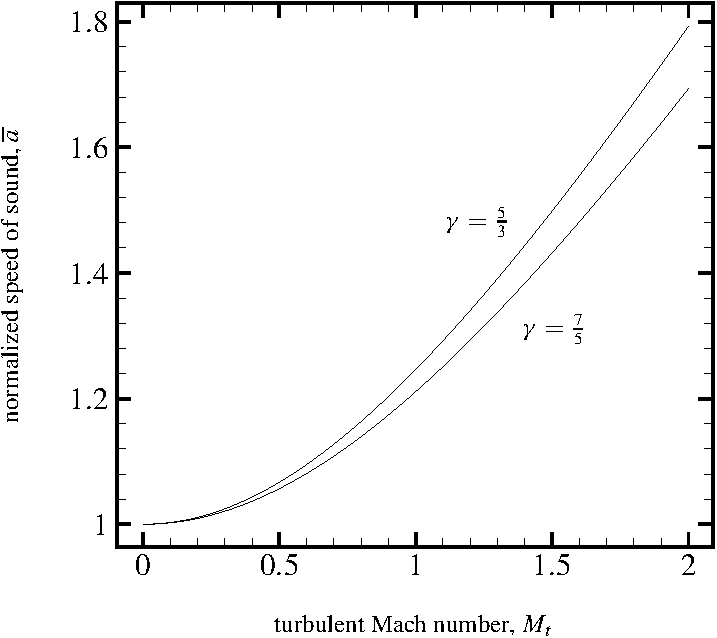
\includegraphics[width=3.36\lengthfigure]{fig3/ParentFig1.pdf}
\caption{Normalized speed of sound $\overline{a}=a/a_{k=0}$
         versus the turbulent Mach number $\Mt=\sqrt{2k}/a_{k=0}$,
         for a calorically perfect gas according to
         Eq.~(\ref{eqn:anorm}).}
\label{fig:anorm-Mturb}
\end{SCfigure}
%

Since the Roe scheme is used to discretize the convection derivatives,
the determination of the eigenstructure of the convective flux Jacobian
$A_i\equiv \partial F_i / \partial Q$ is needed.
It can be checked by substitution that the following definition of $\lambda_i$,
%
\begin{equation}
  \frameeqn{
 \lambda_i=
 \left[
   V_i,~~
   V_i,~~
   \rightarrow,~~
   V_i + a\widehat{X}_i,~~
   V_i - a\widehat{X}_i,~~
   V_i,~~
   V_i
 \right]^{\rm D}
 }~,
 \label{eqn:lambda}
\end{equation}
%
satisfies the necessary relationship ${\rm det}(A_i-w_i I)=0$ (with $w_i$ any element
on the diagonal of $\lambda_i$) and is hence a valid eigenvalue matrix.
Denoting the flow speed by $q$, the non-metric effective speed of sound is found to
be equal to
%
\begin{equation}
  a=\left( P_\rho + \frac{2}{3} k +P_{\rho E} \left( H-q^2-k\right) \right)^{\frac{1}{2}},
  \label{eqn:a}
\end{equation}
%
which as might be expected is a function of the
kinetic energy of turbulence, in contrast to the ``non-turbulent''
speed of sound (here denoted by $a_{k=0}$)
encountered in the eigenstructure of the convection terms of the molecular Navier-Stokes
equations. Dividing both sides of Eq.~(\ref{eqn:a}) by
$a_{k=0}$ and after some reformatting, the normalized speed of sound
can be shown to be equal to
%
\begin{equation}
  \overline{a} \equiv \frac{a}{a_{k=0}}= \left(1+\frac{P_{\rho E}+1}{3} \Mt^2\right)^{\frac{1}{2}},
  \label{eqn:anorm}
\end{equation}
%
where for a calorically perfect gas, $P_{\rho E}+1$ is equal to the ratio of the specific heats,
$\gamma$. Figure \ref{fig:anorm-Mturb} shows the relationship
between $\overline{a}$ and the turbulent Mach number for $\gamma=7/5$
and $\gamma=5/3$.
As the turbulent Mach number increases, its influence on $\overline{a}$
becomes more predominant due to the relative speed of the turbulent
vortices, with respect to the average vortex speed of displacement, gradually
overtaking the thermodynamic sound speed as the information propagation mechanism.
For a perfect or real gas, the derivatives of pressure with respect to the
mass-weighted total energy and density are equal to
%
\begin{equation}
  P_{\rho E}=\bigfrac{1}{\rho \bigfrac{\partial }{\partial P}e(P,\rho)}~~~{\rm and}~~~
  P_{\rho_k}=\left[-\mfd\frac{E-k-q^2}{\rho}- \mfd\frac{\partial e(P,\rho)}{\partial \rho_k} \right]
             \left/ \mfd\frac{\partial e(P,\rho)}{\partial P} \right.~,
\end{equation}
%
with $e$ the internal energy of the gas and where it is assumed that any thermodynamic
property can be obtained from only two others. The partial derivatives involving
the internal energy are to be found with the internal energy written in terms
of the pressure and the partial densities. The right eigenvectors are not unique,
and each column of the matrix can be multiplied by a constant
other than 0; here, we choose the multiplying constant of each column such
as to keep the same units along each row, except for the last column which
is further multiplied by $a^2/\omega$ which is found to result in faster convergence:
%
\begin{equation}
  \frameeqn{
  L^{-1}_i  = \left[
    \begin{array}{@{}c@{}c@{}cc@{}c@{}cccc@{}}
      1      &\cdots  &0      & 0              & \rightarrow &0 & 1 & 0 & 0\alb
      \vdots &\ddots  &\vdots & 0              & \rightarrow &1 & 1 & 0 & 0\alb
      0      &\cdots  &1      & 0              & \rightarrow &1 & 1 & 0 & 0\alb
      v_1 &\cdots&v_d& l_i^{1,1} a  & \rightarrow & v_1 \! +\! \bigfrac{a X_{i,1}}{\widehat{X}_i} & v_1 \! - \! \bigfrac{a X_{i,1}}{\widehat{X}_i} & 0 & 0\alb
      \vdots &\ddots&\vdots& \vdots & \searrow & \vdots & \vdots & \vdots & \vdots\alb
      v_{\nd} &\cdots&v_\nd& l_i^{{\nd},1} a  & \rightarrow & v_{\nd} \! +\! \bigfrac{a X_{i,\nd}}{\widehat{X}_i} & v_{\nd}\! -\! \bigfrac{a X_{i,\nd}}{\widehat{X}_i} & 0 & 0\alb
      q^2\! - \! \bigfrac{P_{\rho_1}}{P_{\rho E}}\!+\!k\phi &\cdots& q^2\! - \! \bigfrac{P_{\rho_\ns}}{P_{\rho E}}\!+\!k\phi   & \sum_{j} l_i^{j,1} a v_j & \rightarrow &  H \! +\!  \bigfrac{a V_i}{\widehat{X}_i}& H \! - \!
         \bigfrac{a V_i}{\widehat{X}_i}  & a^2\phi & 0\alb
      k&\cdots&k& 0 & \rightarrow & k & k & a^2 & 0 \alb
      \omega&\cdots&\omega& 0 & \rightarrow & \omega & \omega & 0 & a^2 \alb
    \end{array}
  \right]
  }
\end{equation}
%
with $\phi=1-2/3 P_{\rho E}$. The exactness of the right eigenvectors can be readily verified by the relation
$\lambda_i = L_i A_i L_i^{-1}$.
Note that the columns of the right eigenvectors containing $l_{i}^{m,n}$ are not needed
in one dimension, while in two dimensions, $l_{i}^{m,n}$ takes on the form
%
\begin{equation}
  l_i^{m,1}= (-1)^{m+1} {X}_{i,m+1}/\widehat{X}_i \, ,
\end{equation}
%
and in three dimensions, becomes,
%
\begin{equation}
  l^{m,1}_i=\frac{{X}_{i,m+2}-{X}_{i,m+1}}{\left[\sum_{j=1}^3 \left( X_{i,j+1}-X_{i,j}\right)^2\right]^{1/2}}
  \, ,~~~~~
  l^{m,2}_i= \frac{ {X}_{i,m+1} l_i^{m+1,1}
        - {X}_{i,m+2} l_i^{m+2,1} }
      { \widehat{X}_i  } \, .
\end{equation}
%
In the above, $\widehat{X}_i$ corresponds to the
magnitude of all derivatives of $X_i$, that is,
%
\begin{equation}
  \widehat{X}_i=\left( \sum_{j=1}^{\nd} X_{i,j}^2\right)^\frac{1}{2}.
\end{equation}
%








\section{Pseudotime relaxation}

Using implicit Euler pseudotime marching the delta form of the discretized
equations can be shown to correspond to
%
\begin{equation}
   \bigfrac{\Delta^n Q}{\Delta \pseudot}
    +\sum_{i=1}^{\nd}\left[ \delta_{X_i}  {\Delta^n F_i}
            - \sum_{j=1}^{\nd} \delta_{X_i}
           \left( K_{i,j} \delta_{X_j}
                 {\Delta^n G}\right) \right]
    -\Delta^n S = -R_{\Delta} \, ,
\label{eqn:deltaform}
\end{equation}
%


\subsection{Block implicit approximate factorization}

To minimize storage requirements and the inversion effort the
LHS of Eq.~(\ref{eqn:deltaform}) is approximated using a multiplication of
one-dimensional operators
based on a block-implicit approximate factorization algorithm
\cite{misc:1955:douglas,misc:1955:peaceman,aiaa:1978:beam,jcp:1977:briley}
and a linearization strategy of the viscous terms by Chang and Merkle \cite{jcp:1989:chang}:
%
\begin{equation}
\left[   \prod_{i=1}^{\nd}
  \left( I+\Delta \pseudot \overline{\delta_{X_i} A_i}
         - \Delta \pseudot \sum_{j=1}^{\nd} \delta_{X_i}
  \left( {K}_{ij}\delta_{X_j} B \right) -\Delta \pseudot \krodel_{1i}  C^{-}\right) \right] \Delta^n Q
        = - \Delta \pseudot R_{\Delta} \, ,
\label{eqn:approxfact}
\end{equation}
%
where $\krodel_{1i}$ is the Kronecker delta,
$B$ the linearization Jacobian of the viscous terms ($B\equiv \partial G / \partial Q$),
and $C^{-}_i$ the linearization Jacobian of the negative source terms
($\partial S^{-} / \partial Q$)
for the $i=1$ sweep but ignored for the other sweeps.
Only the negative source terms are linearized to ensure the stability of the
implicit algorithm \cite{book:1980:patankar} and are set to
%
\begin{equation}
  S^{-}=
  \frac{1}{J} \left[
  \begin{array}{c}
    \vdots\alb
    0\alb
     - \rho k \omega  \alb
     -\frac{5}{6}{\rho k \omega^2}/{\widetilde{k}}
  \end{array}
  \right]
  - \frac{\partial Q}{\partial t} \, .
\end{equation}
%
The term $\overline{\delta_{X_i} A_i}$ is symbolic and
stands for the linearization of the first-order Roe scheme with the Roe Jacobian
locally frozen. The use of a fully linearized Roe scheme is shown in Batten
\etal\ \cite{jcp:1997:batten} not to decrease the number of iterations needed for
convergence for several test problems (in some cases it is even detrimental)
while requiring more work per iteration than the frozen Jacobian approach.
Hence, the equation to solve for each node for the $i$th sweep can be written as
%
\begin{equation}
\frameeqn{
\begin{array}{r}
\left[
  -K^{X_i-\frac{1}{2}}_{ii} B^{X_i-1}
  -\bigfrac{\left( {J^{-1}} L^{-1}  |\lambda|  L \right)_i^{X_i-\frac{1}{2}}}{2 ({J^{-1}})^{X_i-1}}
                         -\frac{A_i^{X_i-1}}{2}
\right] \Delta \widetilde{Q}_i^{X_i-1}
+
\left[ \bigfrac{I}{\Delta \pseudot^{X_i}}-\delta_{i 1} {C^{-}}^{X_i} \right. \alb \left.
+\left( K^{X_i-\frac{1}{2}}_{ii}+K^{X_i+\frac{1}{2}}_{ii} \right)B^{X_i}
  +\bigfrac{\left( {J^{-1}} L^{-1}  |\lambda|  L \right)_i^{X_i-\frac{1}{2}}+
           \left( {J^{-1}} L^{-1}  |\lambda|  L \right)_i^{X_i+\frac{1}{2}}}{2 ({J^{-1}})^{X_i}}
\right] \Delta \widetilde{Q}_i^{X_i}
+ \alb
\left[
  -K^{X_i+\frac{1}{2}}_{ii} B^{X_i+1}
-\bigfrac{\left( {J^{-1}} L^{-1}  |\lambda|  L \right)_i^{X_i+\frac{1}{2}}}{2 ({J^{-1}})^{X_i+1}}
                         +\frac{A_i^{X_i+1}}{2}
\right] \Delta \widetilde{Q}_i^{X_i+1} =
\bigfrac{I}{\Delta \pseudot^{X_i}} {\Delta \widetilde{Q}^{X_i}_{i-1}}
\end{array}
}
\end{equation}
%
where ${\Delta \widetilde{Q}^{X_i}_0}=- \Delta \pseudot^{X_i} R_{\Delta}^{X_i}$
and the total flux increment $\Delta Q^{X_i}$ is set to ${\Delta \widetilde{Q}^{X_i}_{\nd}}$.


It is emphasized that the success of approximate factorization
relies on the degree of invariance of the linearization matrices,
deterring the inclusion of a linearized form of the minmod limiter on
the implicit side. Numerical experiments
show that a ``switch'' type of algorithm on the implicit side
might induce erratic patterns in the convergence history
sometimes preventing a converged solution altogether.
For similar reasons, the implicit treatment of the cross
diffusion terms is not recommended
as their linearization necessarily involves spatial derivatives which are subject
to change from iteration to iteration.



\subsection{Local pseudotime step: CFL condition}

One commonly used acceleration technique is local pseudotime stepping based on
the CFL condition which results in a wave traveling speed of one node per
iteration for convection dominated flows.
However, in multiple dimensions, each dimension assumes a different CFL
condition and one faces the dilemma of specifying a wave
traveling speed proportional to the dimension exhibiting the lowest CFL condition,
commonly referred to as a minimum CFL based local time step, or to the dimension exhibiting the
highest CFL condition which is referred to as a maximum CFL based local time step.
A formulation including both the minimum and maximum CFL based approaches can take the form
%
\begin{equation}
\frameeqn{
\Delta \pseudot = {\rm CFL}
  ~\raisebox{-1.5ex}{$\stackrel{\stackrel{\scriptstyle \nd}{\textstyle \max}}{\scriptstyle i=1}$}
    \left(
      \bigfrac{1}{|V_i|+a \widehat{X}_i}
    \right)^{\sigma}
   \raisebox{-1.5ex}{$\stackrel{\stackrel{\scriptstyle \nd}{\textstyle \min}}{\scriptstyle i=1}$}
    \left(
      \bigfrac{1}{|V_i|+a \widehat{X}_i}
    \right)^{1-\sigma}
}~,
\label{eqn:pseudodt}
\end{equation}
%
where a $\sigma$ varying between 0 and 1 induces a time step of a magnitude situated
respectively between a minimum and a maximum CFL based time step. Unless otherwise
indicated, $\sigma$ is set to 0.5. While it
is acknowledged that for viscous dominated regions, a local time step based
on the Von Neumann number (VNN) would result in a more equitable wave propagation
which might translate into faster convergence, for the purposes of this thesis
Eq.~(\ref{eqn:pseudodt}) is used exclusively.





\section{Boundary conditions}


\begin{figure}
\scalefont{0.5}
\begin{verbatim}
          111111111111111111111111111111111111111111       11111111111111111111111111111111111111111111111
          0++++++++++++++++++++++++++++++++++++++++1       0+++++++++++++++++++++++++++++++++++++++++++++1
          0++++++++++++++++++++++++++++++++++++++++1       0+++++++++++++++++++++++++++++++++++++++++++++1
          0++++++++++++++++++++++++++++++++++++++++1       0+++++++++++++++++++++++++++++++++++++++++++++1
          0++++++++++++++++++++++++++++++++++++++++1       0+++++++++++++++++++++++++++++++++++++++++++++1
          0++++++++++++++++++++++++++++++++++++++++1       0++++++33333333333333+++++++++++++++++++++++++1
          0++++++++++++++++++++++++++++++++++++++++1       0++++++3............3+++++++++++++++++++++++++1
          0++++++++++++++++++++++++++++++++++++++++1       0++++++3............3+++++++++++++++++++++++++1
          0++++++++++++++++++++++++++++++++++++++++1       0++++++3............3+++++++++++++++++++++++++1
          0++++++++++++++++++++++++++++++++++++++++1       0++++++3............3++++33333333333++++++++++1
          33333333333333333333+++++++++++++++++++++1       0++++++3............3++++3.........3++++++++++1
          ...................3+++++++++++++++++++++1       0++++++3............3++++3.........3++++++++++1
          ...................3+++++++++++++++++++++1       0++++++33333333333333++++3.........3++++++++++1
          ...................3+++++++++++++++++++++1       0++++++++++++++++++++++++3.........3++++++++++1
          ...................3+++++++++++++++++++++1       0++++++++++++++++++++++++3.........3++++++++++1
          ...................3+++++++++++++++++++++1       0++++++++++++++++++++++++3.........3++++++++++1
          ...................3+++++++++++++++++++++1       0++++++++++++++++++++++++33333333333++++++++++1
          ...................3+++++++++++++++++++++1       0+++++++++++++++++++++++++++++++++++++++++++++1
          ...................3+++++++++++++++++++++1       0+++++++++++++++++++++++++++++++++++++++++++++1
          ...................3+++++++++++++++++++++1       0+++++++++++++++++++++++++++++++++++++++++++++1
          ...................33333333333333333333331       11111111111111111111111111111111111111111111111
\end{verbatim}
\caption{Examples of the distribution of the node types for
   a backward facing step (left)
   and a two-element airfoil (right); the number ``3'' represents
   a wall condition, ``0'' inflow, ``1'' outflow,
    while ``+'' represents inner nodes and
   ``.'' is used for unactivated nodes.}
\label{fig:BCtypes}
\end{figure}
%


A multiblock stratagem is generally required when tackling
complex geometries with a structured mesh, but it can significantly
complicate the implementation of the domain decomposition algorithms
presented herein for reasons that shall become apparent shortly.
As a substitute to using multiple blocks connected to the geometry
and to one another through their outer edges (or planes in 3D),
any node that is part of the computational domain is allowed to be either
a boundary, inner or inactive node. Although not as multipurpose
as the multiblock, such an approach can be used to solve a wide variety
of flowfields while retaining all the simplicity of a single block.
Figure \ref{fig:BCtypes} shows, for example, how the node types
would be distributed for a backward facing step and a two-element airfoil.

Zeroth order extrapolation polynomials are used to obtain the
properties from the adjacent inner node at the supersonic outflow
boundary (hereafter referred to simply as outflow boundary),
while the properties at the supersonic inflow (hereafter referred to
as inflow), are unaltered in pseudotime. At the symmetry boundary
node, a first order extrapolation polynomial of the form
%
\begin{equation}
  \psi^{X}=\frac{4}{3} \psi^{X+1} - \frac{1}{3} \psi^{X+2} \, ,
  \label{eqn:bdrypolynomial}
\end{equation}
%
is employed to obtain $P^\star$, $k$, $\omega$, $\rho$ and the velocity
components tangent
to the surface, while the perpendicular velocity component is set to zero.
At the wall, the turbulent kinetic energy and the velocity are fixed
to zero, while the effective pressure and temperature (in the case of an
adiabatic wall) are extrapolated as in Eq.~(\ref{eqn:bdrypolynomial}).
Also, the dissipation rate at the wall is specified to
%
\begin{equation}
  \omega_{\rm w}=\frac{36}{5} \frac{\mu}{\rho d_{\rm w}^2} \, ,
\end{equation}
%
with $d_{\rm w}$ the distance between the wall node and its nearest
neighbor. As suggested by Wilcox \cite{book:1994:wilcox}, the freestream value of
the specific dissipation rate is set to
%
\begin{equation}
  \omega_\infty=g_\omega q_\infty
  \label{eqn:g_omega}
\end{equation}
%
with $g_\omega$ given a value of $10 \frac{1}{\rm m}$.


It is well known that an implicit treatment of the boundary
nodes results in less prohibitive restrictions on the pseudotime step size for
some problems, but when solving strong shock waves or other highly non-linear
phenomena it is not uncommon for the time step size to be limited in any case
by the flow physics, even if the time stepping scheme can be shown
to be Von Neumann unconditionally stable (see the chapter on non linear
stability in Laney \cite{book:1998:laney}, for example).
Moreover, experience shows
that treating the boundary conditions presented herein in an
explicit manner does not restrict the size of the local time step more
than implicit boundary conditions would.  For all numerical experiments
presented, an explicit treatment of the boundary nodes is chosen.



\section{Domain Decomposition Algorithms}

\subsection{Standard cycle}

The ``standard cycle'' here implies the usual way of updating the solution
in pseudotime, by first finding the residual for all nodes and then updating
the solution. The algorithm can be written in the following steps:
%
\begin{enumerate}
  \item{update the boundary nodes in the domain\
        \subdomain{\forall i}{X^{\loopS}_i}{X^{\loopE}_i},}
  \item{update the residual in the domain
        \subdomain{\forall i}{X^{\loopS}_i}{X^{\loopE}_i}, }
  \item{update $Q$ (by pseudotime stepping) in \
        the domain \subdomain{\forall i}{X^{\loopS}_i}{X^{\loopE}_i}, and,}
  \item{convergence is attained when $\xi \leq \xiverge$ in the domain \subdomain{\forall i}{X^{\loopS}_1}{X^{\loopE}_1}.}
\end{enumerate}
%



\subsection{Multizone cycle}
\label{section:multizone}

One strategy towards improving the standard cycle is to divide the computational
domain into a number of non-overlapping zones of approximately equal size
and to update in pseudotime only the zones where $\xi>\xiverge$.
This stratagem has been previously employed
by Sawley \etal\ \cite{misc:1994:sawley}
as a convergence acceleration technique for supersonic flows, but where the
computational domain is split into several blocks, instead of several zones.
Note that a ``zone'' is defined as a computational domain region that
can be bounded by boundary and/or inner nodes (see for example Ref.
\cite{jcp:1994:rosenfeld}),
while a ``block'' is defined as a region delimitated  by boundary nodes only.
The zone length in each dimension is set to at most $\phi_1$, a user
specified constant usually given a value of 20.
At each iteration, should the maximum $\xi$ inside each zone be greater
than the user-specified threshold $\xiverge$, the inner nodes up to the
zone boundaries are updated in pseudotime,
followed by the update of the boundary nodes up to the zone boundaries expanded by $\bb$,
and the update of the residual up to the zone boundaries expanded by $\bb+\br$.
The residual and properties of all other nodes of the computational domain
are not altered. Prior to the first iteration,
the computational domain is divided into a number of non-overlapping zones
of length in each dimension no greater than $\phi_1$ with
each zone $z$ defined by the subdomain \subdomain{\forall i}{X^{z,\loops}_i}{X^{z,\loope}_i}.
Then, at each iteration, the following steps are performed:
%
\begin{enumerate}
  \item{for each zone $z$, update $Q$ (by pseudotime stepping) in \
        the subdomain \subdomain{\forall i}{X^{z,\loops}_i}{X^{z,\loope}_i}
	if $\xi > \xiverge$ in the subdomain \subdomain{\forall i}{X^{z,\loops}_i}{X^{z,\loope}_i},}
  \item{for each zone $z$, update the boundary nodes in the subdomain\
        \subdomain{\forall i}{X^{z,\loops}_i-\bb}{X^{z,\loope}_i+\bb}
	if $\xi > \xiverge$ in the subdomain \subdomain{\forall i}{X^{z,\loops}_i}{X^{z,\loope}_i},}
  \item{for each zone $z$, update the residual in the subdomain
        \subdomain{\forall i}{X^{z,\loops}_i-\bb-\br}{X^{z,\loope}_i+\bb+\br}
	if $\xi > \xiverge$ in the subdomain \subdomain{\forall i}{X^{z,\loops}_i}{X^{z,\loope}_i}, and, }
  \item{convergence is attained when $\xi \leq \xiverge$ in the domain \subdomain{\forall i}{X^{\loopS}_1}{X^{\loopE}_1}.}
\end{enumerate}
%
It is noted that the multizone cycle ensures
the residual on all nodes to be up to date after each iteration but,
due to the non self-starting property of this cycle, it is
necessary to compute the residual on the entire domain before the first iteration
is performed.




\section{Numerical experiments}
\label{section:numerical_experiments}

Three steady state supersonic flowfields and one unsteady
flowfield are solved using the different types of cycles
mentioned in the last section, and the performance of each is
assessed on the basis of (i) the number of effective iterations,
(ii) CPU time, and (iii) maximum storage required. To enable a fair
comparison between the different
cycle strategies, the number of effective iterations is defined as
%
\begin{equation}
  {\rm effective~iterations} \equiv
           \frac{\rm number~of~times~an~inner~node~is~updated}
                {\rm total~number~of~inner~nodes} \, ,
  \label{eqn:effiter}
\end{equation}
%
which is a good measure of the cycle performance as long as most of the
computing effort is spent on the pseudotime stepping instead of the
residual, due to the overlap of the residual
determination when a multizone decomposition is used.
The implicit scheme used herein spends three
quarters of its computing effort on the time stepping side, therefore reducing
the residual overlap overhead work and justifying the use of Eq.~(\ref{eqn:effiter})
as a performance parameter. In spite of being accurately measured, the number of
CPU seconds is not regarded as a more meaningful performance parameter due to the
unavoidable bias that might occur in the programming of the cycles and the high
dependence of the work on the architecture of the computer. Certain
enhancements to the multizone cycle, such as unifying adjacent zones, could be implemented which would
result in a non-negligible decrease in work, while the use of a vector
computer (of CRAY type) would advantage the longer loops present in the
standard cycle. Therefore, both the number of effective iterations and CPU time are
monitored for all test cases.






\subsection{Inviscid supersonic inlet with a blunt leading edge}

%
\begin{figure}[!b]
   \fontsizefigure
   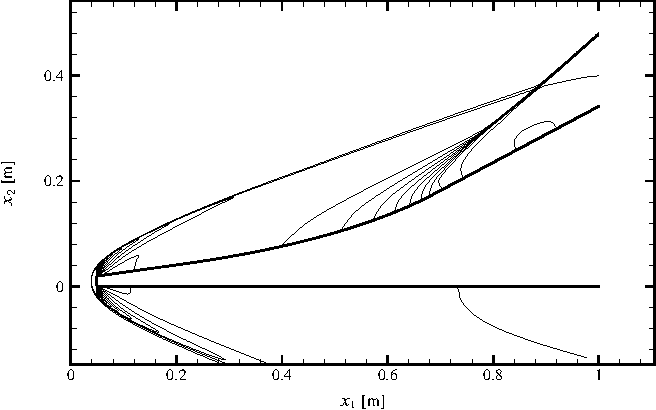
\includegraphics[width=6.3\lengthfigure]{fig3/ParentFig6.pdf}
\caption{Closeup of the pressure contours for the blunt leading edge inviscid supersonic inlet
         case obtained using a $512 \times 256$ grid;
         the inflow conditions correspond to $M=5$, $P=4$ kPa and $T=240$ K;
         no difference is noticeable between the pressure contours obtained
         with the different cycles.}
\label{fig:inlet-P}
\end{figure}
%





A first comparison between the different cycles is performed for a steady-state
inviscid flow over a 1~m long supersonic inlet. Air enters the channel at a Mach
number of 5, a pressure of 4~kPa, and a temperature of 240~K. The grid
size is varied between $128 \times 64$ nodes and $512 \times 256$
nodes. The user-defined parameters of interest are set to (when applicable)
%
\begin{displaymath}
 \sigma=0.5,~~~ \xiverge=100~\frac{1}{\rm s},~~~ \varphiverge=5000~\frac{1}{\rm s},
          ~~~\phi_0=4, ~~~ \phi_1=20, ~~~\phi_2=3, ~~~{\rm and}~~~\phi_3=9,
\end{displaymath}
%
where the value of 0.5 given to $\sigma$ translates into a geometric average
between the minimum CFL condition based pseudotime step and the maximum CFL
condition based pseudotime step. The convergence threshold $\xiverge$ is low
enough that a decrease in $\xiverge$ would not result in any noticeable
difference of the pressure contours in Figure \ref{fig:inlet-P}, except for the
active domain cycle, as pointed out later. It is noted that the use of
the entropy correction by Yee \etal\ \cite{jcp:1990:yee} with $\widetilde{\zeta}=0.2$
is here used to avoid a carbuncle
phenomenon near the shock formed by the blunt leading edge.

Table \ref{tab:inlet} shows the CPU time and effective
iterations needed to reach convergence for the marching window,
marching window / multizone, active domain, multizone, and
standard cycles. Due to the $\CFL=1$ restriction  on the traveling speed
of the waves in the flowfield to approximately one grid line per iteration,
the standard cycle requires a number of iterations proportional to the
number of grid lines along the streamwise direction, \ie\ 293 iterations
for a $128 \times 64$ mesh to 1391 iterations for a $512 \times 256$ mesh. The multizone
cycle suffers the same symptoms but has the extra advantage of \emph{not} allocating
work to the zones where all nodes exhibit a $\xi$ smaller than the user
specified threshold, therefore reducing the computing to a smaller and smaller domain
as the iteration count progresses and the non-converged flow region moves towards
the domain exit. This results in impressive savings in iteration count of
1.8 times for the coarse mesh and of 4.4 times for the fine mesh.
Both the active domain cycle and the marching window cycle decrease further the
iteration count by allowing a
computational window to travel in space following the propagation of the waves.
This results in a decrease in effective iterations, compared to the standard cycle
using the $512 \times 256$ mesh,
of 14 and 16 times for the active domain and marching window respectively.
Furthermore, the use of multizone decomposition inside the marching window
focuses the pseudotime stepping effort to the regions requiring more iterations
to reach convergence, such as the region of subsonic flow upstream of the
inlet blunt leading edge, hence resulting in only 45 effective iterations to
reach convergence and an overall reduction in effective iterations of
31 times compared to the standard cycle.
%
\begin{table}
  \fontsizetable\center
  \begin{threeparttable}
  \tablecaption{Effective iteration count, work, and storage comparison
                 for the blunt leading edge inviscid supersonic
                inlet case.\tnote{a}}
  \label{tab:inlet}
  \begin{tabular}{c@{~~~~~~}r@{.}lr@{.}lr@{.}lcr@{.}lr@{.}lr@{.}l}
    \toprule
                          &\mc{6}{c}{$128\times 64$ nodes}
                            &&\mc{6}{c}{$512\times 256$ nodes}  \\
    \cmidrule(lr){2-7}\cmidrule(lr){9-14}
    cycle                 &\mc{2}{c}{iter.}& \mc{2}{c}{work} & \mc{2}{c}{stor.}
                            &&\mc{2}{c}{iter.}& \mc{2}{c}{work} & \mc{2}{c}{stor.}\\
    \midrule
    marching window / multizone    &   34&4       &    1&0         &  0&11
                                  &&   44&9       &   22&2       &  0&91 \\

    marching window                &   40&4       &    1&1         &  0&11
                                  &&   86&8       &   38&9       &  0&91 \\

    active domain                  &   55&6       &    1&3        &  0&10
                                  &&   102&2      &   39&2       &  0&81 \\

    multizone                      &   158&5      &    3&8        &  1&0
                                  &&   318&6      &  131&6      &  16&0  \\

    standard cycle                 &   293&0      &    6&5        &  1&0
                                  &&   1391&0     &  524&3      &  16&0  \\
    \bottomrule
  \end{tabular}
  \begin{tablenotes}
    \item[a] At a CFL number of unity.
  \end{tablenotes}
  \end{threeparttable}
\end{table}
%

It is reminded that the standard cycle, the multizone cycle, and
the marching window cycle (with and without multizone decomposition)
all guarantee that
%
\begin{displaymath}
  \xi \leq \xiverge ~\forall~ {\rm inner~nodes} \, ,
\end{displaymath}
%
once convergence is reached
[as previously stated],
which is a necessary condition for a well-posed acceleration technique.
The latter is \emph{not} a property
of the active domain method when the discretization stencil for the
streamwise convection derivative depends on downstream nodes
in locally supersonic flow. The Yee TVD limiter used
here has this property, and the active domain
algorithm induces a converged residual that does not satisfy the convergence
criterion of Eq.~(...).

It could be argued that raising the CFL number would improve the standard
cycle over the others for this particular case. Investigation on a change of
CFL number is not performed, but is addressed in the subsequent test problems.
It is noted that for many realistic problems dominated by non linear phenomena,
nonlinear stability conditions restrict the use of high CFL numbers until the waves
have started to settle down considerably and for which the use
of a fine mesh results in very poor performance of the standard cycle.



